\section{Proof of Theorem~\ref{thm:all}}\label{sec:proofall}

Let $\epsilon(m,x_0)=\epsilon_{\rm main}+\epsilon_{\rm miss}+\epsilon_{rs}+\epsilon_T+\epsilon_{\gamma\ge2}+\epsilon_{K_2}+\epsilon_{K_3}$ be the sum of the bounds of Section~\ref{sec:errors}, where $\epsilon_{K_j}$ denote the right sides of \eqref{eq:XK2} and \eqref{eq:XK3} with the tails included.

\begin{theorem}\label{thm:cert}
Put $x_0(m)=\sqrt{500}/m$ for $3\le m\le7$ and $x_0(m)=1$ for $8\le m\le100$. Then
\[
\epsilon\big(m,x_0(m)\big)\le0.347\qquad(3\le m\le100),
\]
with the largest value at $m=8$; for $3\le m\le7$ one has $\epsilon\le0.0025$.
\end{theorem}

\begin{proof}
Every term of $\epsilon(m,x_0)$ is a finite sum of explicit quantities, which we evaluate in ball arithmetic with $96$ bits \cite{Joh17}. Bessel functions are evaluated by Arb's certified routines, the suprema in \eqref{eq:Xmain} by the exact critical points, and the solutions of \eqref{eq:deltaeq} are enclosed as described after \eqref{eq:XT}. The values are listed in Appendix~\ref{app:margins} and plotted in Figure~\ref{fig:certificate}; the computation takes about twelve minutes.
\end{proof}

\begin{theorem}\label{thm:analytic}
For every $m\ge101$, $\epsilon(m,1)\le0.3382$.
\end{theorem}

\begin{proof}
\emph{Leading family and missing pairs.} Group the pairs by $S$. For $1\le S\le m+1$, Lemma~\ref{lem:deltas} gives $S-\eta_-=S(2m-S)/(2m+4)\ge(2m-1)/(2m+4)>1/\pi$, so Lemma~\ref{lem:mainS} applies, and the pairs with $a+b+2=S$ contribute at most $p_2(S)u^S\varphi(S,m)$, where $p_2(S)=\sum_{a+b=S-2}d_1(a)d_1(b)$. Missing pairs have $S\ge m/2+2$ and contribute at most $p_2(S)u^S$. For $S>300$ we use, for the pairs in $\mathcal L_m$, $|\rho_{a,b}-e^{-\pi xS}|\le e^{-\pi\Delta_s}+e^{-\pi S}\le2e^{-\pi S(m-1)/(2m+4)}\le2e^{-0.485\pi S}$ (Lemma~\ref{lem:deltas}(iv)), and $p_2(S)\le P(q)^2q^{-S}$ with $q=e^{-0.4\pi}$, so these terms add up to at most $2P(q)^2\varrho^{301}/(1-\varrho)$ with $\varrho=e^{-0.485\pi}/q$. Evaluated in ball arithmetic, the total is at most $0.33815$ for every $101\le m\le300$, the largest value being at $m=101$.

For $m>300$ we compare with $m=300$. The bound $\eta_-$ decreases in $m$; for $S\le3$ one checks $\eta_+=0$ (for $S=3$ this is $\sqrt{1+4/m}+\sqrt{1-2/m}\ge2$, true for $m\ge3$), and for $S\ge4$ the function $\sqrt{m(m+4)}-\sqrt{m(m+4-2S)}=2S/\big(\sqrt{1+4/m}+\sqrt{1+(4-2S)/m}\big)$ decreases in $m$; $y_t=\pi\sqrt{m(m+4-2S)}$ increases, and $8S/m$ decreases. Hence $\varphi(S,m)\le\varphi(S,300)$ whenever $2S\le304$. For $152<S\le300$ the term $\varphi(S,300)$ has $\epsilon_1=1$ and $\min(1,\pi\eta_+)=1$, so again $\varphi(S,m)\le\varphi(S,300)$. The missing pairs for $m>300$ have $S\ge m/2+2>152$, and their terms $p_2(S)u^S$ with $S\le300$ are counted at $m=300$; those with $S>300$ are in the tail. So the bound at $m=300$, which is $0.1090$, holds for all $m>300$.

\emph{The other pieces.} By Lemmas~\ref{lem:rsbig}, \ref{lem:g2big} and~\ref{lem:mockbig}, with $q=q(101)$ (since $c$ increases with $m$, the bound with $q(101)$ holds for all $m\ge101$),
\[
|\mathcal X_{rs}|+|\mathcal X_T|\le3.02\cdot10^{-8},\quad|\mathcal X_{\gamma\ge2}|\le3\cdot10^{-45},\quad|\mathcal X_{K_2}|\le6\cdot10^{-79},\quad|\mathcal X_{K_3}|\le7\cdot10^{-77}
\]
at $m=101$. Each bound decreases in $m$: in Lemma~\ref{lem:rsbig} the factor $(2m+1)^2e^{-\pi m/4}$ decreases for $m\ge101$ and $g_0$ increases; in Lemma~\ref{lem:g2big} the factor $e^{-\pi\sqrt{t_0}/2}$ dominates; in Lemma~\ref{lem:mockbig} the exponent $2\pi\sqrt{2m+2}+z_1-z_0\le2\pi\sqrt{2m+2}+2\pi\sqrt m-\pi m$ decreases.
\end{proof}

\begin{figure}[t]
\centering
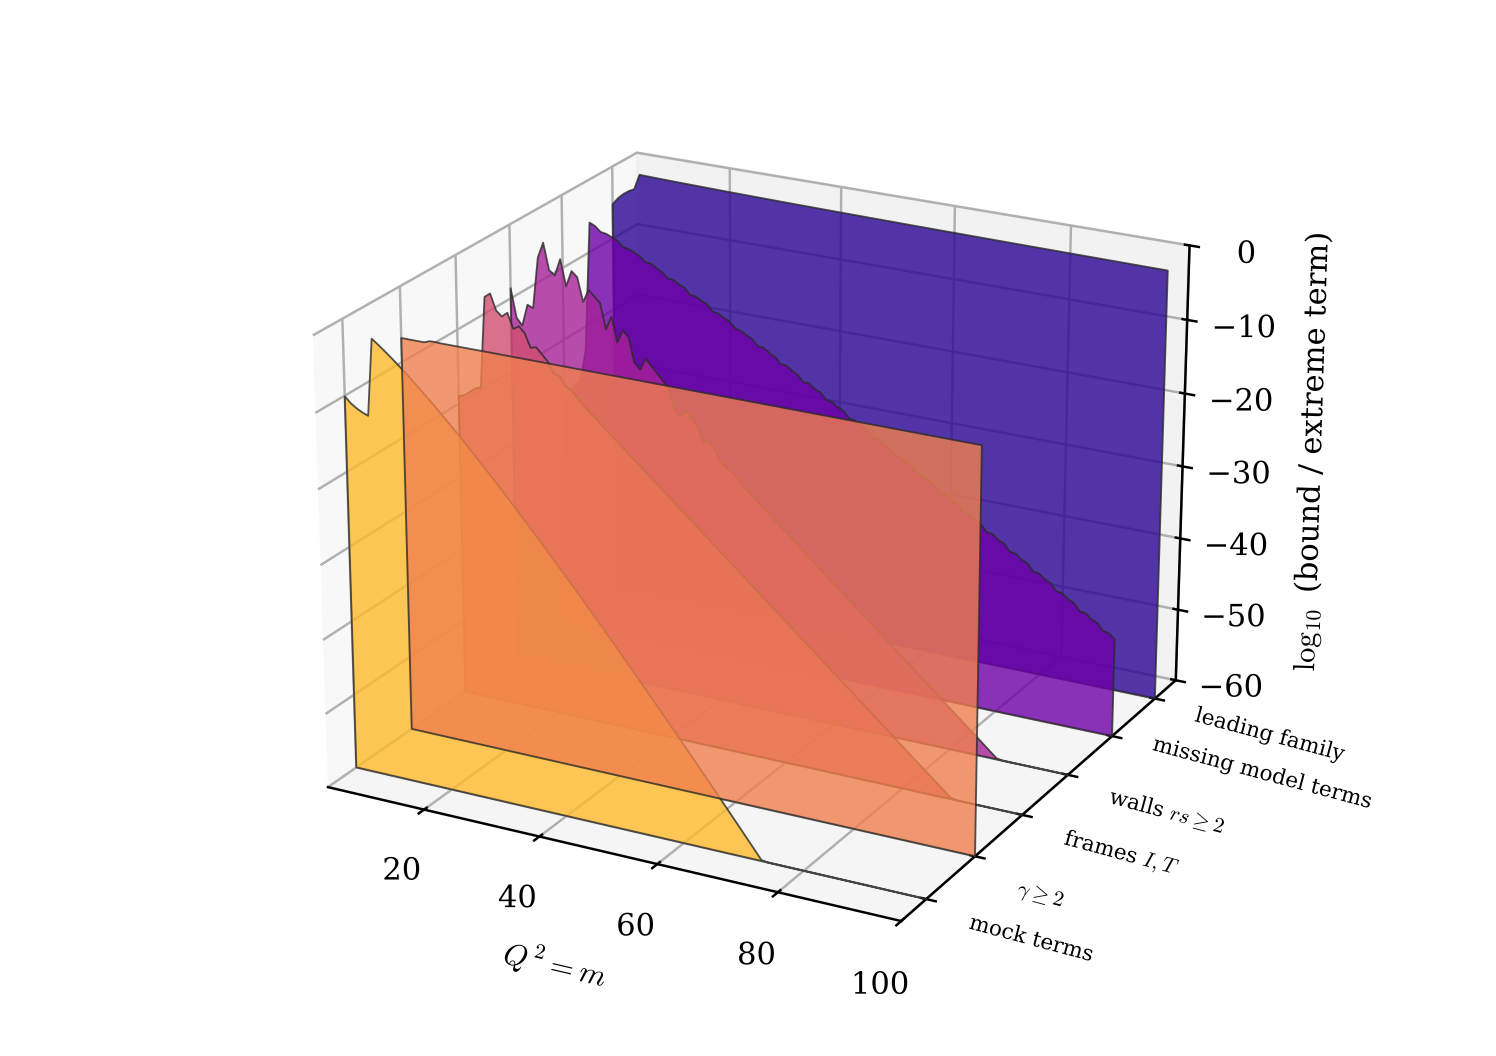
\includegraphics[width=0.84\textwidth]{fig_certificate.png}
\caption{The pieces of the certificate for $3\le Q^2\le100$, on a logarithmic scale and divided by the extreme term $\mathcal E$: shadow terms, terms with $\gamma\ge2$, the frames $I,T$, the walls with $rs\ge2$, the missing model terms and the error of the leading family. Only the last one matters numerically; the others are below $10^{-2}$ at $Q^2=8$ and fall off quickly.}\label{fig:certificate}
\end{figure}

\begin{figure}[t]
\centering
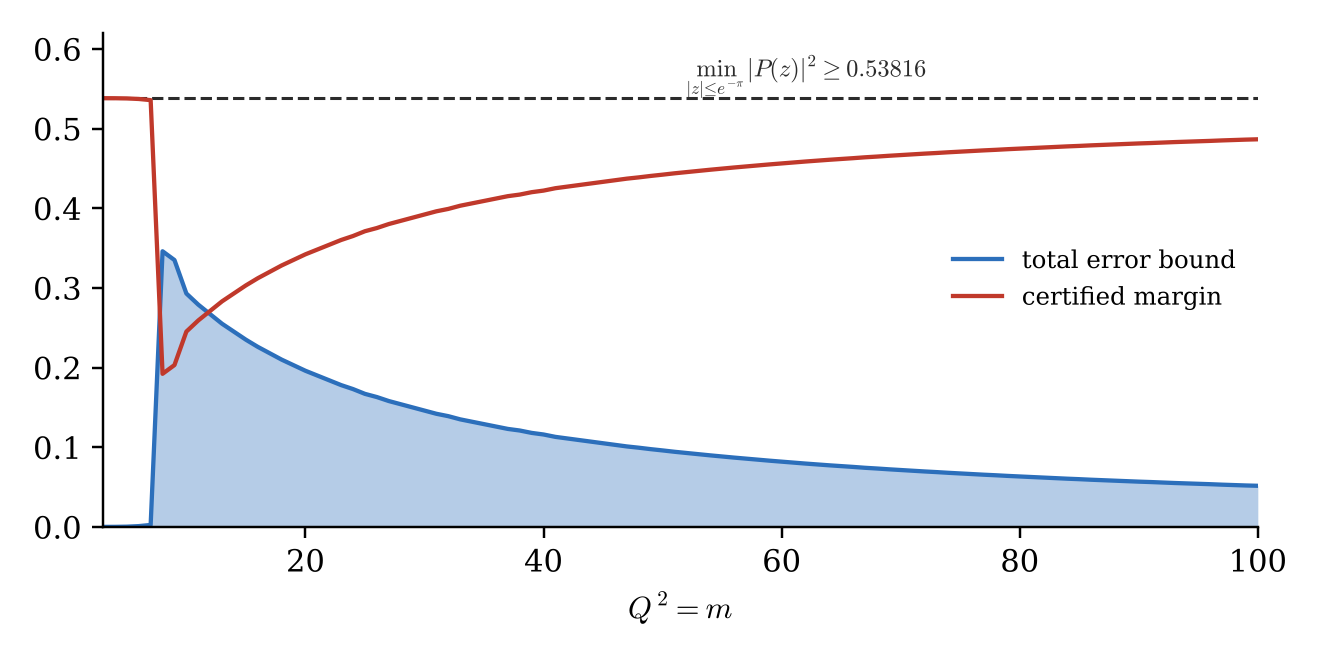
\includegraphics[width=0.8\textwidth]{fig_margins.png}
\caption{The total error bound $\epsilon(m,x_0(m))$ and the margin $0.53816-\epsilon$ for $3\le Q^2\le100$. The margin is smallest at $Q^2=8$, where it is $0.19$.}\label{fig:margins}
\end{figure}

\begin{proof}[Proof of Theorem~\textup{\ref{thm:all}}]
By Proposition~\ref{prop:reduction} it suffices to prove $d^*(m,n,\ell)>0$ for reduced charges. For $m=1,2$ this is Theorem~\ref{thm:main}. Let $m\ge3$. If $m\le7$ and $D\le500$, it is Theorem~\ref{thm:bounded}. Otherwise $x=\sqrt D/m\ge x_0(m)$, with $x_0(m)$ as in Theorem~\ref{thm:cert} for $m\le100$ and $x_0=1$ for $m\ge101$. By \eqref{eq:decomp} and the bounds of Section~\ref{sec:errors}, which are uniform in $x\ge x_0$ and in $\ell$,
\[
\frac{d^*(m,n,\ell)}{\mathcal E(D,m)}\ \ge\ |P(z)|^2-\epsilon(m,x_0)\ \ge\ 0.53816-0.347>0
\]
by Proposition~\ref{prop:pmin} (note $|z|=e^{-\pi x}\le e^{-\pi}$) and Theorems~\ref{thm:cert} and~\ref{thm:analytic}. Since $\mathcal E(D,m)>0$, $d^*(m,n,\ell)>0$.
\end{proof}

\begin{corollary}\label{cor:asym}
Under Hypothesis~\textup{\ref{hyp:R}}, for every reduced charge with $m\ge3$,
\[
0.19\,\mathcal E(D,m)\ \le\ d^*(m,n,\ell)\ \le\ 2.51\,\mathcal E(D,m).
\]
In particular $\log d^*(Q,P)=\pi\sqrt{1+4/Q^2}\,\sqrt{D}-4\log D+O_{Q^2}(1)$ as $D\to\infty$ with $Q^2$ fixed, and $\log d^*=\pi\sqrt{Q^2P^2-(Q\cdot P)^2}+O(\log D)$ when $Q^2\to\infty$ with $\sqrt D/Q^2$ bounded, the Bekenstein--Hawking entropy of the black hole.
\end{corollary}

\begin{proof}
The lower bound is the proof above. For the upper bound, $|P(z)|^2\le P(e^{-\pi})^2\le2.156$ and $\epsilon\le0.347$. The asymptotics follow from \eqref{eq:ext}, $I_\nu(y)\sim e^y/\sqrt{2\pi y}$, and $\pi\sqrt D\,(\sqrt{1+4/m}-1)\le2\pi\sqrt D/m$.
\end{proof}

\begin{remark}\label{rem:sharp}
The minimum $0.5389$ of Proposition~\ref{prop:pmin} is reached in the limit: as $m\to\infty$ along charges with $x=1$ and $\ell=m$ odd, $z=-e^{-\pi}$, and the bounds in the proof of Theorem~\ref{thm:analytic} tend to $0$, since $\varphi(S,m)\to0$ for each fixed $S$. So, under Hypothesis~\ref{hyp:R}, $d^*/\mathcal E$ comes arbitrarily close to $0.5389$, and the factor of the leading family cannot be replaced by a single term; the dominance argument of \cite{Ros24}, with one dominant term, does not carry over to level two without the resummation of Theorem~\ref{thm:model}.
For moderate charges the picture is already accurate: at $Q^2=3$, $P^2/2=10$, $Q\cdot P=3$ the exact index gives $d^*/\mathcal E=0.9485$ while $|P(z)|^2=0.9910$, and at $Q^2=4$, $P^2/2=58$, $Q\cdot P=4$ the two numbers are $0.99990$ and $0.99999$.
\end{remark}
